\documentclass[12pt,a4paper,english]{article}
\usepackage{times}
\usepackage[utf8]{inputenc}
\usepackage{babel,textcomp}
\usepackage{mathpazo}
\usepackage{mathtools}
\usepackage{amsmath,amssymb}
\usepackage{ dsfont }
\usepackage{listings}
\usepackage{graphicx}
\usepackage{float}
\usepackage{subfig} 
\usepackage[colorlinks]{hyperref}
\usepackage[usenames,dvipsnames,svgnames,table]{xcolor}
\usepackage{textcomp}
\definecolor{listinggray}{gray}{0.9}
\definecolor{lbcolor}{rgb}{0.9,0.9,0.9}
\lstset{backgroundcolor=\color{lbcolor},tabsize=4,rulecolor=,language=python,basicstyle=\scriptsize,upquote=true,aboveskip={1.5\baselineskip},columns=fixed,numbers=left,showstringspaces=false,extendedchars=true,breaklines=true,
prebreak=\raisebox{0ex}[0ex][0ex]{\ensuremath{\hookleftarrow}},frame=single,showtabs=false,showspaces=false,showstringspaces=false,identifierstyle=\ttfamily,keywordstyle=\color[rgb]{0,0,1},commentstyle=\color[rgb]{0.133,0.545,0.133},stringstyle=\color[rgb]{0.627,0.126,0.941},literate={å}{{\r a}}1 {Å}{{\r A}}1 {ø}{{\o}}1}

% Use for references
\usepackage[sort&compress,square,comma,numbers]{natbib}
\DeclareRobustCommand{\citeext}[1]{\citeauthor{#1}~\cite{#1}}

% Fix spacing in tables and figures
%\usepackage[belowskip=-8pt,aboveskip=5pt]{caption}
%\setlength{\intextsep}{10pt plus 2pt minus 2pt}

% Change the page layout
%\usepackage[showframe]{geometry}
\usepackage{layout}
\setlength{\hoffset}{-0.6in}  % Length left
\setlength{\voffset}{-0.8in}  % Length on top
\setlength{\textwidth}{480pt}  % Width
\setlength{\textheight}{680pt}  % Height
%\setlength{\footskip}{25pt}

\newcommand{\VEV}[1]{\langle#1\rangle}
\title{FYS-STK 4155 Project 2}
\date{}
\author{ Kristoffer Langstad \footnote{\url{https://github.com/krilangs/FYS-STK4155}}\\ \textit{krilangs@uio.no}}

\begin{document}%\layout
\maketitle
\begin{abstract}
In this project we use classification and regression to analyze two data sets. For classification we study the Taiwan credit card data for default payment from the UCI Machine Learning Repository \cite{UCI} as a binary classification problem. This data set contains some errors which we remove before the data are scaled and trained for further analysis. Here we use logistic regression and multilayer perceptron neural networks to do the analysis by calculating the accuracy score of the results we get from these methods. The results are then compared between the two methods, and compared with a similar study on the same data from a scientific article by \citet{origarticle}. For the regression analysis, we create a data set by using the Franke function. This function have already been analyzed in a earlier project \cite{proj1} with linear regression. Here we do the regression analysis by using the multilayer perceptron neural network from the classification case by changing the cost function. The following results are used to calculate the $R^2$ score, which are compared with the previous project $R^2$ score and the accuracy score for the other results we have gotten in this project. To get the best results we tune a few parameters to find the best learning rate $\gamma$ and regularization parameter $\lambda$. For the classification we found that the neural network (NN) is better than the logistic regression of the credit card data. The logistic regression gave an accuracy score of around 0.714, while the neural network gave an accuracy score of around 0.795 with best $\lambda=1.286\cdot10^{-4}$ and $\gamma=5.829\cdot10^{-2}$. This fits well with the results in the scientific paper which concluded that the NN is better for classification than logistic regression. For the regression analysis of the Franke data for the same parameters as in the previous project, $n_x=n_y=50$ and $\sigma=0.2$ which are number of grid points in x- and y-direction and the standard deviation, the linear regression with ordinary least squares (OLS) gave the best $R^2$ score of around 0.681 while the NN regression gave around 0.551 with best $\lambda=1.841\cdot10^{-10}$ and $\gamma=1.582\cdot10^{-4}$. So for the same parameters the linear regression is better than the NN regression.
\end{abstract}

\section{Introduction}
\label{sect:Intro}
A much used method in statistical analysis is classification. With this type of method we can sort large amount of data and predict outcomes of different situations. In classification there are several methods which can be used, and some work better than others in different types of scenarios. We will look at the two classification methods logistic regression and neural network analysis in this project.

In this project we will develop our own logistic regression code for classification using Python to study credit card data from Taiwan taken from the UCI Machine Learning Repository \cite{UCI}. Since this data set has been previously studied in a scientific research paper by \citet{origarticle} considering data mining techniques, we will use the results in the article to compare with our results. We will also develop our own multilayer perceptron (MLP) code and neural network code (NN), with a stochastic gradient descent solver and different cost functions depending on the case to be solved. With these methods we will classify the credit card data with logistic regression and neural network. Then we solve a regression problem of a data set by the Franke function by using the neural network code adapted to regression. For the Franke function we compare with results from a previous project for solving the regression problem using linear regression \cite{proj1}.

First we will look at the data sets to be evaluated in this project. This includes the Taiwan credit card data (classification) and the Franke function (regression). Then in the theory section, we look at the theory of the different methods and algorithms to be used in this project, which are implemented into Python programs for solving the classification and regression problems. In the methods section we go through how we set up and implement the codes for solving the classification and regression cases. We start by downloading and reading in the credit card data. This data set is then altered to account for missing and/or wrongly implemented values before the remaining data are scaled and trained. Then we create the Logistic Regression class with a stochastic gradient descent solver and cost function to being able to reproduce the results in the scientific article \cite{origarticle}. Then we create a Feed Forward Neural Network code with back propagation and a new cost function by training the network to find optimal weights and biases. We test different regularization parameters and learning rates to find the optimal accuracy score. Then we use the Neural Network code with appropriate cost function to perform a regression analysis on the Franke function data. In the Results section we compare and discuss the results we get from the Logistic Regression and Neural Network analysis for classification, and do an evaluation of the regularization parameters and learning rates. Then we compare and discuss the results from the previous regression project for the Franke function and the regression analysis with Neural Network. In the conclusion section we come up with a critical evaluation of the various algorithms we have used in this project. From this evaluation we conclude on which algorithm works best for the classification case and which is best for the regression case.

\section{Data}
\label{sect:Data}
\subsection{Classification: Credit Card Data}
\label{subsect:credit_data}
The classification analysis in this project is of the Taiwan default payments credit card data downloaded from the UCI \cite{UCI} as an .xls file. The outcome of the default payment is binary as YES=1, NO=0. The original data set contains 30 000 number of instances (720 000 data points) with 23 explanatory variables/attributes (24 with the output) explained on the web site as:
\begin{enumerate}
	\item X1: Amount of the given credit (NT dollar): it includes both the individual consumer credit and his/her family (supplementary) credit. 
	\item X2: Gender (1 = male; 2 = female). 
	\item X3: Education (1 = graduate school; 2 = university; 3 = high school; 4 = others). 
	\item X4: Marital status (1 = married; 2 = single; 3 = others). 
	\item X5: Age (year). 
	\item X6 - X11: History of past payment. We tracked the past monthly payment records (from April to September, 2005) as follows: X6 = the repayment status in September, 2005; X7 = the repayment status in August, 2005; . . .;X11 = the repayment status in April, 2005. The measurement scale for the repayment status is: -1 = pay duly; 1 = payment delay for one month; 2 = payment delay for two months; . . .; 8 = payment delay for eight months; 9 = payment delay for nine months and above. 
	\item X12-X17: Amount of bill statement (NT dollar). X12 = amount of bill statement in September, 2005; X13 = amount of bill statement in August, 2005; . . .; X17 = amount of bill statement in April, 2005. 
	\item X18-X23: Amount of previous payment (NT dollar). X18 = amount paid in September, 2005; X19 = amount paid in August, 2005; . . .;X23 = amount paid in April, 2005. 
\end{enumerate}
By analysis of the data set; there are errors that have to be taken into consideration where there are values that does not correspond to the values that should be given from the variables description above for X2-X4. Also remove instances with zeros only for past bill statements or paid amounts for X12-X23. The remaining data of the first 23 attributes are set as the design matrix \textbf{X}, and the outputs are in the vector \textbf{y}.

\subsection{Regression: Franke's function}
\label{subsect:franke_data}
In the regression analysis in this project we evaluate the two-dimensional Franke function which is defined as:
\begin{align}
\label{eq:Franke_func}
f(x,y)=&\frac{3}{4}\exp\left(-\frac{(9x-2)^2}{4}-\frac{(9y-2)^2}{4}\right)+
\frac{3}{4}\exp\left(-\frac{(9x+1)^2}{49}-\frac{(9y+1)^2}{10}\right)\\ 
+& \frac{1}{2}\exp\left(-\frac{(9x-7)^2}{4}-\frac{(9y-3)^2}{4}\right)- \frac{1}{5}\exp\left(-(9x-4)^2-(9y-7)^2\right) \nonumber
\end{align}
This function is defined for $x,y\in[0,1]$, and is a widely used function for testing various interpolation and fitting algorithms. With this function we also add a normally distributed noise $\epsilon\sim \mathcal{N}(0,\sigma^2)$ so the total function for making the data is
\begin{equation*}
F(x,y)=f(x,y)+\epsilon.
\end{equation*}
For easy comparison with the earlier project \cite{proj1} we use a standard deviation $\sigma=0.2$ and $n_x=n_y=50$ number of grid points in the x- and y-directions each which are the same as in the previous project. We also test with a smaller standard deviation of $\sigma=0.1$ with the same number of grid points and with $n_x=n_y=100$ and $\sigma=0.1$ to see the affect on the results. In the previous project, the Franke function was evaluated with linear regression methods like the ordinary least squares (OLS) calculating among other the $R^2$ score. For more information on the linear regression on the Franke function, see the previous project \textit{FYS-STK 4155 Project 1} \cite{proj1}.

\section{Theory}
\label{sect:Theory}
\subsection{Regression}
\label{subsect:Regression}
For the regression evaluation we will look at the $R^2$ score to evaluate the performance of the model as
\begin{equation}
\label{eq:R2_score}
R^2(\textbf{y},\tilde{\textbf{y}})=1-\frac{\sum_{i=0}^{n-1}(y_i-\tilde{y})^2}{\sum_{i=0}^{n-1}(y_i-\bar{y})^2},
\end{equation}
with model $\tilde{\textbf{y}}$ and the mean value, $\bar{y}$, of the data \textbf{y} as
\[\bar{y}=\frac{1}{n}\sum_{i=0}^{n-1}y_i.\]
A $R^2$ score of 1 is the optimal value, which defines a perfect fit between the model and true values.

\subsection{Classification}
\label{subsect:Classification}
For the classification we will measure the performance of the model with the accuracy score as
\begin{equation}
\label{eq:accuracy_score}
\text{Accuracy}=\frac{\sum_{i=1}^{n}I(t_i=y_i)}{n},
\end{equation}
with target $t_i$, model output $y_i$, number of targets $n$ and indicator function $I$ as
\[I=\begin{cases}
1, \text{ if } t_i=y_i\\
0, \text{ if } t_i\neq y_i
\end{cases}.\]
The optimal accuracy score is 1 as for the $R^2$ score for regression. With the accuracy score we can easily calculated the error rate, as in the scientific article \cite{origarticle}, as:
\begin{equation}
\label{eq:error_rate}
\text{error rate}=1-\text{accuracy score}
\end{equation}

\subsection{Logistic Regression (LR)}
\label{subsect:LR}
In logistic regression we use linear regression in $x$ to model the posterior probabilities with sums in the domain [0,1]. Logistic regression is what is called a soft classifier. This means that it outputs the probability of a given category. For our case with logistic regression, the output is a binary case which gives either 1 if the credit card user could default the credit card debt or 0 if not. The probability that a data point $x_i$ belongs to a specific category $y_i$ can be represented by the likelihood given by the logistic (Sigmoid) function as
\begin{equation}
\label{eq:sigmoid}
p(\textbf{x})=\frac{e^{\hat{\beta}\textbf{x}}}{1+e^{\hat{\beta}\textbf{x}}},
\end{equation}
where $\hat{\beta}=[\beta_0,\beta_1,...,\beta_p]$ are the weights/predictors we want to extract from the data and $\textbf{x}=[1,x_1,x_2,...,x_p]$ is the design matrix. The probabilities for the binary case have the following relation:
\begin{equation*}
p(y_i=0|x_i,\hat{\beta})=1-p(y_i=1|x_i,\hat{\beta})
\end{equation*}

\subsubsection{Maximum Likelihood Estimation (MLE)}
\label{subsect:MLE}
For the total likelihood for all the possible outcomes from a given dataset $\mathcal{D}=\{(y_i, x_i)\}$ with binary variables $y_i\in\{0,1\}$, that are independent and identically distributed (i.i.d.), we use the MLE principle to maximize the probability of seeing the observed data:
\begin{equation}
\label{eq:max_likelihood}
P(\mathcal{D}|\hat{\beta})=\prod_{i=1}^{n}\left[p(y_i=1|x_i,\hat{\beta})\right]^{y_i}\left[1-p(y_i=1|x_i,\hat{\beta})\right]^{1-y_i}
\end{equation}
From this likelihood we get the log-likelihood as:
\begin{equation}
\label{eq:log_likelihood}
P_{\log }(\hat{\beta})=\log[P(\mathcal{D}|\hat{\beta})]=\sum_{i=1}^{n}\left(y_i\log[p(y_i=1|x_i,\hat{\beta})]+(1-y_i)\log[1-p(y_i=1|x_i,\hat{\beta})]\right)
\end{equation}

\subsubsection{Cost function/cross-entropy}
\label{subsect:Cost_func}
For the classification problem we define the cost function as the negative of the log-likelihood as 
\begin{align}
\label{eq:cost_func}
\mathcal{C}(\hat{\beta})=-P_{\log }(\hat{\beta})= -\sum_{i=1}^{n}\left(y_i\log[p(y_i=1|x_i,\hat{\beta})]+(1-y_i)\log[1-p(y_i=1|x_i,\hat{\beta})]\right).
\end{align}
Maximization of the log-likelihood is then the same as minimizing the cost function. In statistics the cost function is also called the cross-entropy. Rewriting of the cost function (eq. \ref{eq:cost_func}) the leads to:
\begin{equation}
\label{eq:cost_func_rewritten}
\mathcal{C}(\hat{\beta})=-\sum_{i=1}^{n}\left(y_i(\textbf{x}_{i*}\hat{\beta})-\log(1+e^{\textbf{x}_{i*}\hat{\beta}})\right).
\end{equation}

The $\hat{\beta}$ parameters are found through minimization of the cost function by taking the derivative of the cost function (eq. \ref{eq:cost_func_rewritten}) with respect to the $\hat{\beta}$ values. Define vector $\textbf{y}\in\mathcal{R}^n$ for $n$ elements $y_i$, matrix $\textbf{X}\in\mathcal{R}^{n\times p}$ with $x_i$ values and vector $\textbf{p}\in\mathcal{R}^n$ for fitted probabilities $p(y_i|x_i,\hat{\beta})$ with non-linear dependence on $\hat{\beta}$. The minimized cost function becomes
\begin{equation}
\label{eq:min_cost_func}
\frac{\partial \mathcal{C}(\hat{\beta})}{\partial \hat{\beta}}=-\textbf{X}^T(\textbf{y}-\textbf{p}).
\end{equation}
This gives set of linear equations to solve the system for $\hat{\beta}$. Define diagonal matrix \textbf{W} with elements $p(y_i|x_i,\hat{\beta})(1-p(y_i|x_i,\hat{\beta}))$. The second derivative of the cost function, also called the Hessian matrix, is then in compact form:
\begin{equation}
\label{eq:Hessian}
\frac{\partial^2 \mathcal{C}(\hat{\beta})}{\partial \hat{\beta}\partial \hat{\beta}^T}=\textbf{X}^T\textbf{W}\textbf{X}.
\end{equation}

The resulting equation of minimization of the cost function is non-linear, and have to be solved using minimization algorithms called gradient descent methods.

For the multilayer perceptron (MLP) (sect. \ref{subsect:MLP}), the cost function can be rewritten in terms of the weights $\textbf{W}$, biases $\textbf{b}$ and activation function $f(\textbf{z})$ as
\begin{equation}
\label{eq:cost_MLP}
\mathcal{C}(\textbf{W},\textbf{b})=-\sum_{j=1}^{n}t_j\log(p(y_j|z_j))+(1-t_j)\log(1-p(y_j|z_j)).
\end{equation}

For the regression problem the cost function we choose to use is defined as
\begin{equation}
\label{eq:C_reg}
\mathcal{C}=\frac{1}{2}\sum_{i=1}^{n}(t_i-a^L_i)^2.
\end{equation}
The minimization for this cost function is
\begin{equation}
\label{eq:C_reg_deriv}
\frac{\partial \mathcal{C}}{\partial a^L_i}=t_i-a^L_i.
\end{equation}


\subsection{Gradient Descent (GD)}
\label{sect:GD}
As stated in the cost function section (\ref{subsect:Cost_func}), we will use gradient descent methods to optimize the cost function by its minimum. In GD the $\hat{\alpha}$ parameters are adjusted iteratively to the largest negative value of the gradient for a given number of iterations or until a given tolerance is reached. This is calculated as
\begin{equation}
\label{eq:GD_general}
\hat{\alpha}^{(n+1)}=\hat{\alpha}^{(n)}-\gamma\nabla_{\hat{\alpha}} \mathcal{C}(\hat{\alpha}^{(n)}),
\end{equation}
where $\gamma$ is a learning rate parameter which acts as a hyperparameter for controlling the step length. Since the cost function is to be optimized with optimal $\hat{\alpha}_{\text{opt}}$ parameters, then there is an optimal $\gamma_{\text{opt}}$ value. If $\gamma<\gamma_{\text{opt}}$, then the GD may take a long time or not even converge within the time frame or for the given number of iterations. If $\gamma>\gamma_{\text{opt}}$, then the GD may not find the minimum value/$\hat{\alpha}_{\text{opt}}$ that we want.

For logistic regression (LR) we have $\hat{\alpha}=\hat{\beta}$, such that the optimal $\hat{\beta}_{\text{opt}}$ values becomes
\begin{equation*}
\label{eq:GD}
\hat{\beta}_{\text{opt}}^{(n+1)}=\hat{\beta}_{\text{opt}}^{(n)}-\frac{\partial \mathcal{C}(\hat{\beta}^{(n)})}{\partial \hat{\beta}}\left[\frac{\partial^2 \mathcal{C}(\hat{\beta}^{(n)})}{\partial \hat{\beta}\partial \hat{\beta}^T}\right]^{-1}=\hat{\beta}^{(n)}_{\text{opt}}-\gamma\frac{\partial \mathcal{C}(\hat{\beta}^{(n)})}{\partial \hat{\beta}},
\end{equation*}
which can be rewritten to
\begin{equation}
\label{eq:GD_LR}
\hat{\beta}_{\text{opt}}^{(n+1)}=\hat{\beta}_{\text{opt}}^{(n)}-(\textbf{X}^T\textbf{W}\textbf{X})^{-1}(\textbf{X}^T(\textbf{p}-\textbf{y}))=\hat{\beta}_{\text{opt}}^{(n)}-\gamma(\textbf{X}^T(\textbf{p}-\textbf{y})).
\end{equation}

For the MLP (sect. \ref{subsect:MLP}) we have the parameter $\hat{\alpha}$ as the weights \textbf{W} and biases \textbf{b}.

For regression and ordinary least square (OLS) we have $\hat{\alpha}=\hat{\beta}$, which gives
\begin{equation}
\label{eq:GD_OLS}
\hat{\beta}_{\text{OLS}}^{(n+1)}=\hat{\beta}_{\text{OLS}}^{(n)}-(\textbf{X}^T\textbf{X})^{-1}(\textbf{X}^T(\textbf{x}\hat{\beta}^{(n)}-\textbf{y})).
\end{equation}

Some important things to notice about the standard GD is that; it is sensitive to initial conditions $\hat{\beta}^{(0)}_{\text{opt}}$ and choices of learning rates, it treats all directions in the parameter space uniformly, it can misinterpret a local minimum as a global minimum and normally the gradient is computationally expensive to calculate for large datasets. To improve the calculations we introduce another gradient descent method; stochastic gradient descent (STD) with mini-batches. The mini-batches are a subset of the data to take the gradient on. So use stochasticity on the gradient descent on randomly picked mini-batches with sizes $M$. This gives a chance that to not use the entire dataset, and the stochasticity can increase the possibility of finding the global minimum and not a local minimum. For $n$ data points there will be $n/M$ mini-batches, which are denoted by $B_k$ with $k=0,1,...,n/M$.

\subsection{Neural Networks (NN)}
\label{sect:NN}
Much of the theory about neural networks are from \citet{hastie2009} ch.11 and \citet{morten_NN}. Neural networks are computational models that are supposed to mimic biological systems, and they consist of layers of nodes that are connected. Neural networks can be used in both regression and classification problems. Neural networks have, as seen in Figure \ref{fig:Neural_network}, an input layer, a hidden layer and an output layer. This is a simple case with two input variables/nodes, one hidden layer with 4 nodes and one node in the output layer. Neural networks can contain many hidden layers, and the number of nodes in each layer have to be decided by us and may vary from layer to layer. The input and output layers contain as many nodes as there are input and output variables respectively. The number of output variables vary depending on the problem and may differ from the number of input variables. From the figure we see that the input variables are sent to the hidden layer nodes where they are processed with an activation function before sent to the output layer. The connection between the nodes are affected by weight variables $w$ which gives weighted sums to be passed through the activation function. The outputted weighted sum have to pass a certain threshold to not give zero output.

\begin{figure}[htbp]
	\centering\includegraphics[width=0.3\linewidth]{Neural_network.png}
	\caption{Schematic diagram of a simple single hidden layer, feed-forward neural network with two input nodes, four nodes in the single hidden layer and one output node.\label{fig:Neural_network}}
\end{figure} 

\subsubsection{Multilayer perceptron (MLP)}
\label{subsect:MLP}
Figure \ref{fig:Neural_network} shows a feed-forward neural network (FFNN) where the information only moves in one direction through the layers, as seen by the arrows. If all the nodes in a layer is connected to all the other nodes in the next layer, we call it a fully-connected FFNN. When there are three or more layers in the network with non-linear activation function on the nodes, then we call the network a multilayer perceptron (MLP).

The output \textbf{y} is produced with the activation function $f(\textbf{z})$ as
\[\textbf{y}=f(\textbf{Wx}+\textbf{b}),\]
with the activation 
\[\textbf{z}=\textbf{Wx}+\textbf{b},\]
where \textbf{W} are the weights, \textbf{x} are the inputs and \textbf{b} are biases in the nodes. The activation for the $i$-th node in the $l$-th layer is given as
\[z_i^l=\sum_{j=1}^{M}W^l_{ij}x_j+b_i,\]
with $M$ the number of possible inputs in node $i$ in layer $l$. The output of all the nodes in the $l$-th layer is
\[y_i^l=f^l\left(\sum_{j=1}^{N_{l-1}}W_{ij}^ly_j^{l-1}+b_i^l\right),\]
with $N_l$ the number of nodes in layer $l$.

\subsubsection{Back propagation}
\label{subsect:back_prop}
The weights and biases have to be optimized to decrease the error. This leads to the back propagation algorithm. The optimization is done by minimizing the cost function $C$ with respect to the weights and biases at the output layer $l=L$:
\begin{align*}
\frac{\partial \mathcal{C}(\textbf{W},\textbf{b})}{\partial W^L_{jk}}&=\begin{cases*}
f^{\prime}(z^L_j)a_k^{L-1}(a^L_j-t_j), \text{ for Regression}\\
f^{\prime}(z^L_j)a_k^{L-1}\frac{a^L_j-t_j}{a^L_j(1-a^L_j)}, \text{ for Classification}
\end{cases*}\\
\frac{\partial \mathcal{C}(\textbf{W},\textbf{b})}{\partial b^L_{j}}&=\delta_j^L
\end{align*}
$t_j$ are the targets as in the accuracy score equation \ref{eq:accuracy_score}. The output error $\delta^L$ is defined as:
\begin{equation*}
\delta_j^L=f^{\prime}(z^L_j)\frac{\partial \mathcal{C}(\textbf{W},\textbf{b})}{\partial a^L_j}
\end{equation*}
For the back propagation through the hidden layers, $l=L-1,L-2,...,2$, the back propagation error is computed before the weights and biases are updated at each layer:
\begin{align*}
\delta_j^l&=\sum_{k}\delta_k^{l+1}W_{kj}^{l+1}f^{\prime}(z^l_j)\\
W_{jk}^l&\leftarrow W_{jk}^l-\gamma\frac{\partial \mathcal{C}(\textbf{W},\textbf{b})}{\partial W_{jk}^l}= W_{jk}^l -\gamma \delta_j^la_k^{l-1} \\
b^l_j&\leftarrow b^l_j-\gamma\frac{\partial \mathcal{C}(\textbf{W},\textbf{b})}{\partial b_j^l}=b^l_j-\gamma\delta_j^l
\end{align*}
The parameter $\gamma$ is a learning rate parameter as in the gradient descent section (\ref{sect:GD}). From these equations it is clear that they the cost function $\mathcal{C}$ and the activation function $f(\textbf{z})$ should be differentiable.

\subsubsection{Weights and biases}
\label{subsect:W_b}
The biases are initialized with a small value equal to 0.01. This could have been set to zero, but having a small value makes sure that all nodes have a small output. The weights are initialized from a uniform distribution with $n$ number of nodes in the input layer: \[W_{ij}\in\frac{1}{\sqrt{n}}[-1,1].\]

\subsubsection{Activation function}
\label{subsect:activ_func}
When choosing the activation function, there are some properties that it has to follow. The activation function should be continuous, it should be non-constant and reach saturation on the range ends and quickly change at the middle. There are several functions we could choose from. A very popular function is the sigmoid function in equation \ref{eq:sigmoid}, which is the one we are using in this project. This is effective for classification cases, but not for regression. So for the regression case, we choose a linear output activation function (at the output layer $l=L$) equal to \[f(z^L_i)=\sum_{j=1}^{N_{l-1}}W_{ij}^ly_j^{l-1}+b_i^l.\]  

\subsubsection{Regularization parameter}
\label{subsect:regular_param}
Neural networks are often prone to overfitting as a cause of having many parameters. To account for this we introduce a regularization with a $L_2$ term on the weights (looks like Ridge regression). The cost function now with the regularization parameter $\lambda$ becomes:
\begin{align*}
\mathcal{C}&\rightarrow\mathcal{C}+\lambda||\textbf{W}||^2_2\\
\frac{\partial \mathcal{C}}{\partial \textbf{W}}&\rightarrow \frac{\partial \mathcal{C}}{\partial \textbf{W}}+\lambda\textbf{W}
\end{align*}

\subsection{Parameter tuning}
\label{subsect:tuning}
We have choose the hyperparameters to use in the calculations. This could be done manually by testing different values for the parameters. This is not a very efficient way. What we are doing is to use a random search to find the best hyperparameters. We use a Scikit-Learn class in Python called \textit{RandomizedSearchCV}. This is run for 100 hyperparameter samples using 5 folds for cross-validation for every sample. We also choose a set number of epochs equal to 300. The class evaluates the model on the training data for every parameter using the cross-validation to avoid overfitting. Then we end up with a best model to be evaluated with the test data.

For the logistic regression with a stochastic gradient solver we choose a set batch size equal to 200, which is normally a default value. So in this case we only have to find the learning rate with the randomized search. The neural network has several hyperparameters on the other hand. The batch size is also set to 200 here for simplicity. We will use two hidden layers, where the first layers contains 100 nodes and the second layers contains 50 nodes. The only hyperparameters left are then the learning rate and the regularization parameter.

\section{Methods}
Start by first downloading the credit card data from the UCI Machine Learning Repository \cite{UCI} as an Excel file "\textit{default of credit card clients.xls}". The credit card data set is explained in the Data section \ref{subsect:credit_data}. The data set contains values that don't correspond to the given value explanations in the Data section. For the ID's in the data set that has these values that don't fit in, we simply exclude them from the analysis. Then we split the remaining data into training and test sets where 28\% are test data and the remaining are training data using Scikit-Learn functions in Python. To avoid favoring of a model which in all cases predicts the outcome as non-default, we upsample the number of default payment samples in the training set. We use a random oversampler function from the \textit{imblearn} library to randomly duplicate the default payment till equal number of default and non-default samples. These new data are then preprocessed by scaling and centering. The values are centered by subtracting the mean of the continuous variables in the training data for both the training and test data. The continuous variables in the training and test data are scaled by the standard deviation in the training set. After scaling then the preprocessed data are stored separately for training and test data as "\textit{.npz}" files, and exported to the Data folder.

Now we start making the Logistic Regression code. The aim for this code is to reproduce the LR analysis in the scientific report by \citet{origarticle}. Since this is a classification problem we use the cross-entropy in equation \ref{eq:cost_func_rewritten} as the cost function. We use the stochastic gradient descent in equation \ref{eq:GD_LR} with mini-batches, which is explained in section \ref{sect:GD}, to calculate the optimal parameters $\hat{\beta}$ for the given cost function. To find the optimal $\beta$ values, we need to find the optimal learning rate $\gamma$, which is explained in the parameter tuning section \ref{subsect:tuning}. The optimal $\beta$ parameters are then stored, and used to produce the cumulative number of target data as function of number of data for the best theoretical curve, modeled curves for default and not default payment and the diagonal baseline curve to be plotted. With this we also calculate the area ratio for the two model cases as the area between the model curve and baseline curve divided by the area between the theoretically best curve and baseline curve with optimal value 1, and the error rate in equation \ref{eq:error_rate}. The best model is when the model curve is close to the best curve, which is greater than the baseline \cite{origarticle}. We also calculate the accuracy score in equation \ref{eq:accuracy_score} which we will use to compare with the other methods later.

Next is to create the neural network (NN) code with multilayer perceptron network (MLP) and back propagation, which is explained in section \ref{sect:NN}. For this case we train the network to find the optimal weights and biases in the cost function in equation \ref{eq:cost_MLP} with the sigmoid (eq. \ref{eq:sigmoid}) activation function. As for with logistic regression, we need the best values for the learning rate $\gamma$ and regularization parameter $\lambda$ (sect. \ref{subsect:tuning}). After training the network we calculate the area ratios, error rates and accuracy scores to compare with the results from the LR code and the NN analysis in the scientific report \cite{origarticle}. We also test the MLP class for overfitting data.

Next we will use the NN code on the regression case for fitting the Franke function data in equation \ref{eq:Franke_func} discussed in section \ref{subsect:franke_data}. Now the cost function is defined as in equation \ref{eq:C_reg}. Once again we find the best regularization and learning rate parameters to calculate the parameters $\hat{\beta}$ as discussed in the parameter tuning section \ref{subsect:tuning}. After finding these optimal parameters, we now calculate the $R^2$ score in equation \ref{eq:R2_score}. We then compare our NN regression results with the results obtained in project 1 \cite{proj1} for the Franke function.

Now that we are done with all the calculations, we summarize and evaluate the algorithms we have used to find out which is best for the classification case and which is best for the regression case.

\section{Results}
\label{sect:Results}
\subsection{Classification}
\label{subsect:result_class}
In Table \ref{tab:logreg} we see the area ratios, accuracy scores, error rates, best learning rate and best regularization parameter for LR and NN in the classification case. In Figure \ref{fig:class_best_params} we see visualizations for the accuracy scores for LR and NN as functions of the learning rate and the regularization parameter. The best values are the combinations of the parameters that maximizes the accuracy scores in the sub-figures. These values are found numerically as explained in the parameter tuning section \ref{subsect:tuning}, and can be seen in Table \ref{tab:logreg}. In Figure \ref{subfig:LR_best} we see that the accuracy score drops for higher and lower learning rates. In Figure \ref{subfig:NN_best} we see that the accuracy score drops for lower learning rate values, and that the regularization parameter stays about the same when it is not bigger than $\approx10^{-2}$. So it looks like the accuracy score is more dependent on the learning rate than on the regularization parameter (when it is not bigger than $\approx10^{-2}$ at least).

In Figure \ref{fig:class_lift_charts} we see lift charts for LR and NN. There we see the cumulative gains as functions of the number of samples for the best model, default, not default and baseline. By looking at the figures we see that the models does worse when predicting the not default than the default, as seen by the area ratios in Table \ref{tab:logreg}. We see that the figure for NN (fig. \ref{subfig:NN_chart}) has a curve for default that is closer to the best model than in the figure for LR (fig. \ref{subfig:LR_chart}). This means that the area ratio is better for NN than LR, which corresponds well with the area ratio values we have in Table \ref{tab:logreg}. So NN seems to be a better fit to the credit card data, at least for higher number of samples. For up to around 20\% of the data, then the two models seems to be about the same at least by eye.

If we compare the default area ratios we got in Table \ref{tab:logreg} and the ones in the scientific paper \cite{origarticle}, we see that they are close to each other where the validation area ratios in the paper are 0.44 (LR) and 0.54 (NN). So the NN is better at predicting the default of the credit card user than the LR. Both methods are somewhat good at predicting the positive outcome, but they are not that good at predicting the negative outcome which is the area ratio on the not default of the credit card user. The CPU time for finding the hyperparameters with the randomized cross-validation (sect. \ref{subsect:tuning}) was about 3.5 minutes for LR and about 43 minutes for NN. This is because the LR only is dependent on one hyperparameter, while NN is dependent on two. So the NN has many more parameters to run through. Even though the NN model is more computer heavy, the results with this model are better than for LR such that the NN model should benefit us. 

If we compare the error rates we got in Table \ref{tab:logreg} and the ones in the scientific paper, we see that the error rates in the paper are much better than what we got with our calculation. So they got much better error rates, but our area ratios are quite similar too each other. The reason for this may be that we have different parameters that affect the results of the accuracy score, but not the area ratios. Since the paper does not include the input parameters, it is not that easy to conclude what the differences are.

\begin{table}[htbp!]
	\centering
	%\hspace{-1cm}
	\begin{tabular}{ |c|c|c| }
		\hline \rule{0pt}{13pt}
		 & Logistic Regression & Neural Network \\
		\hline \rule{0pt}{13pt}
		Area ratio default & 0.470462 & 0.566069  \\
		\hline \rule{0pt}{13pt}
		Area ratio not default & 0.131816 & 0.158604 \\
		\hline \rule{0pt}{13pt}
		Accuracy score (train) & 0.680867 & 0.715727 \\
		\hline \rule{0pt}{13pt}
		Accuracy score (test) & 0.713843 & 0.794770 \\
		\hline \rule{0pt}{13pt}
		Error rate (train) & 0.319133 & 0.284273 \\
		\hline \rule{0pt}{13pt}
		Error rate (test) & 0.286157 & 0.205230 \\
		\hline \rule{0pt}{13pt}
		Best learning rate, $\gamma$ & 4.450669$\cdot10^{-3}$ & 5.829307$\cdot10^{-2}$ \\
		\hline \rule{0pt}{13pt}
		Best regularization parameter, $\lambda$ & - & 1.285610$\cdot10^{-4}$ \\
		\hline
	\end{tabular}	
	\caption{Table for classification case for logistic regression and neural network on the credit card data. From this table we see that neural network give higher and better area ratios and accuracy scores. This means that neural network is a better fit to the credit card data for classification. The CPU time for finding the hyperparameters with the randomized cross-validation (sect. \ref{subsect:tuning}) was about 3.5 minutes for LR and about 43 minutes for NN.
	\label{tab:logreg}}
\end{table}
\begin{figure}[htbp]
	%\hspace*{-2.5cm}
	\subfloat[This is a plot of the accuracy score for the training and validation data for the credit card data as a function of the learning rate for logistic regression. This is a visualization of how to find the best learning rate value to be used in the logistic regression. This best value is actually found numerically. Here we see that the best value is around $\gamma=10^{-3}$.\label{subfig:LR_best} ]{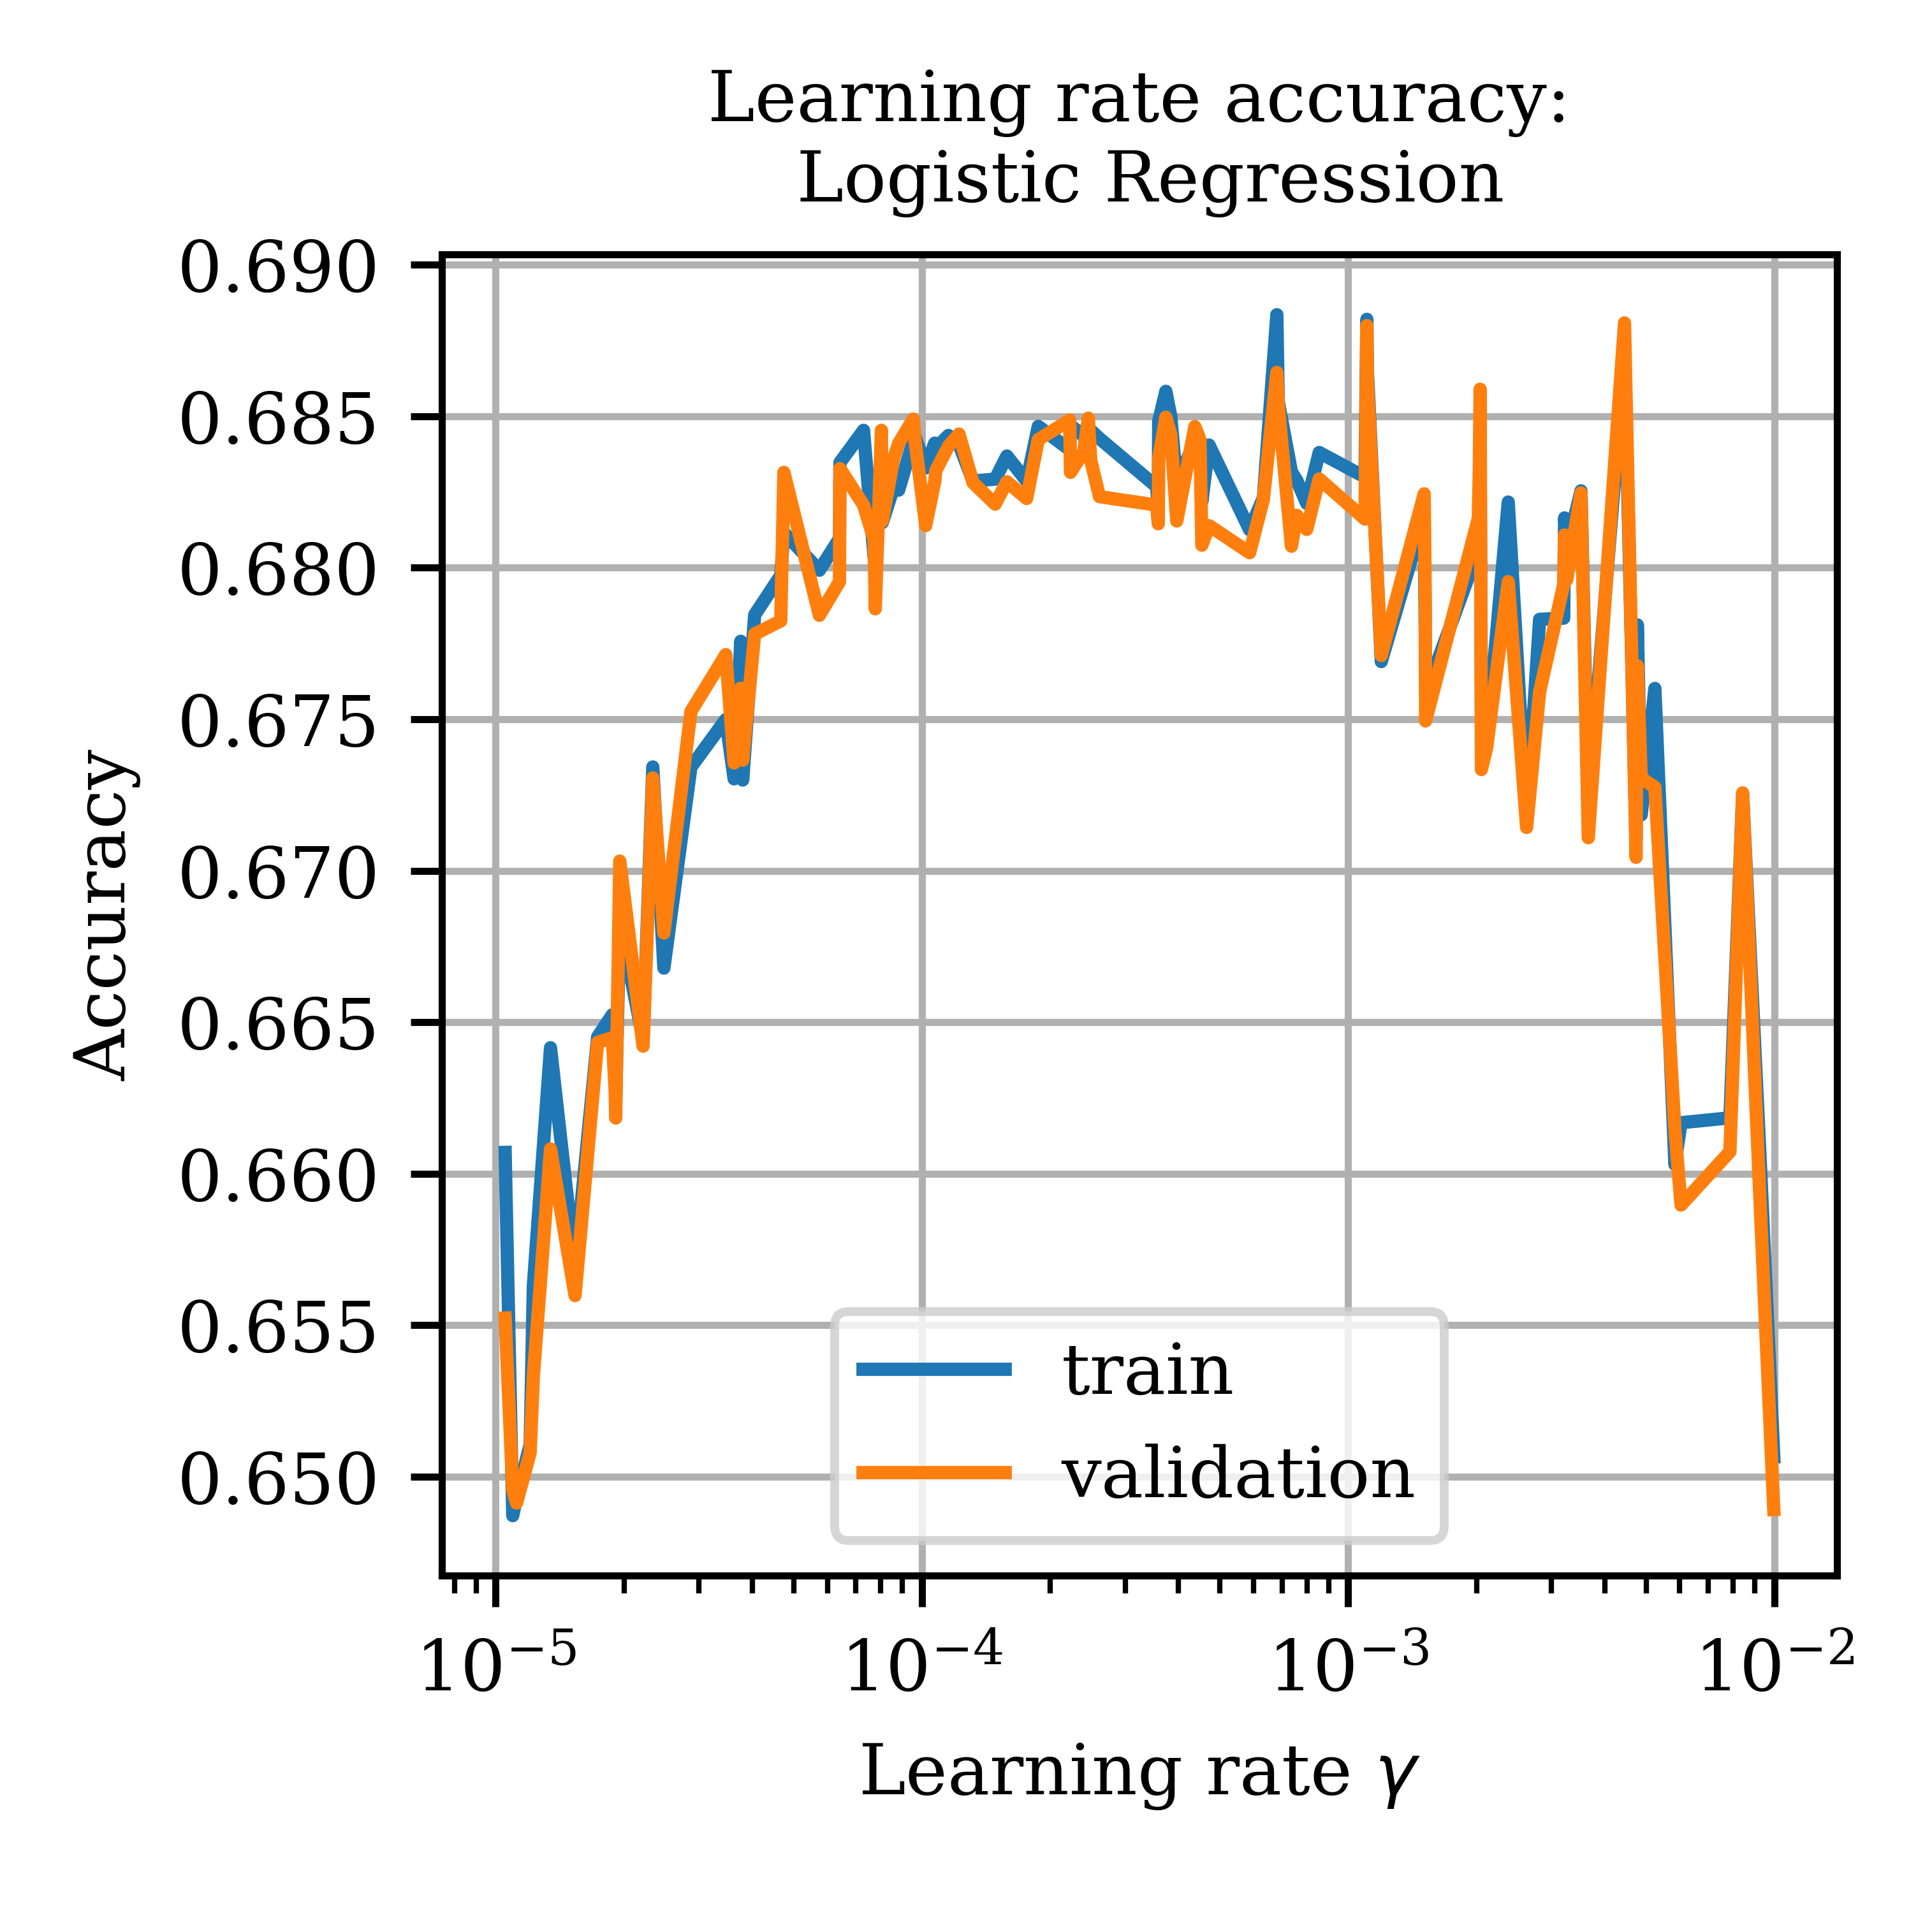
\includegraphics[width=0.5\linewidth]{logreg_learning_rate_accuracy.png}}
	\hspace{0.5em}
	\subfloat[Here we see a heatmap for the validation accuracy for the neural network classification case as function of the regularization parameter and learning rate. This is a visualization of how to find the best learning rate and best regularization parameter to be used in the neural network. Here we see that the best values are around $\lambda=10^{-4}$ and $\gamma=5\cdot10^{-2}$.\label{subfig:NN_best} ]{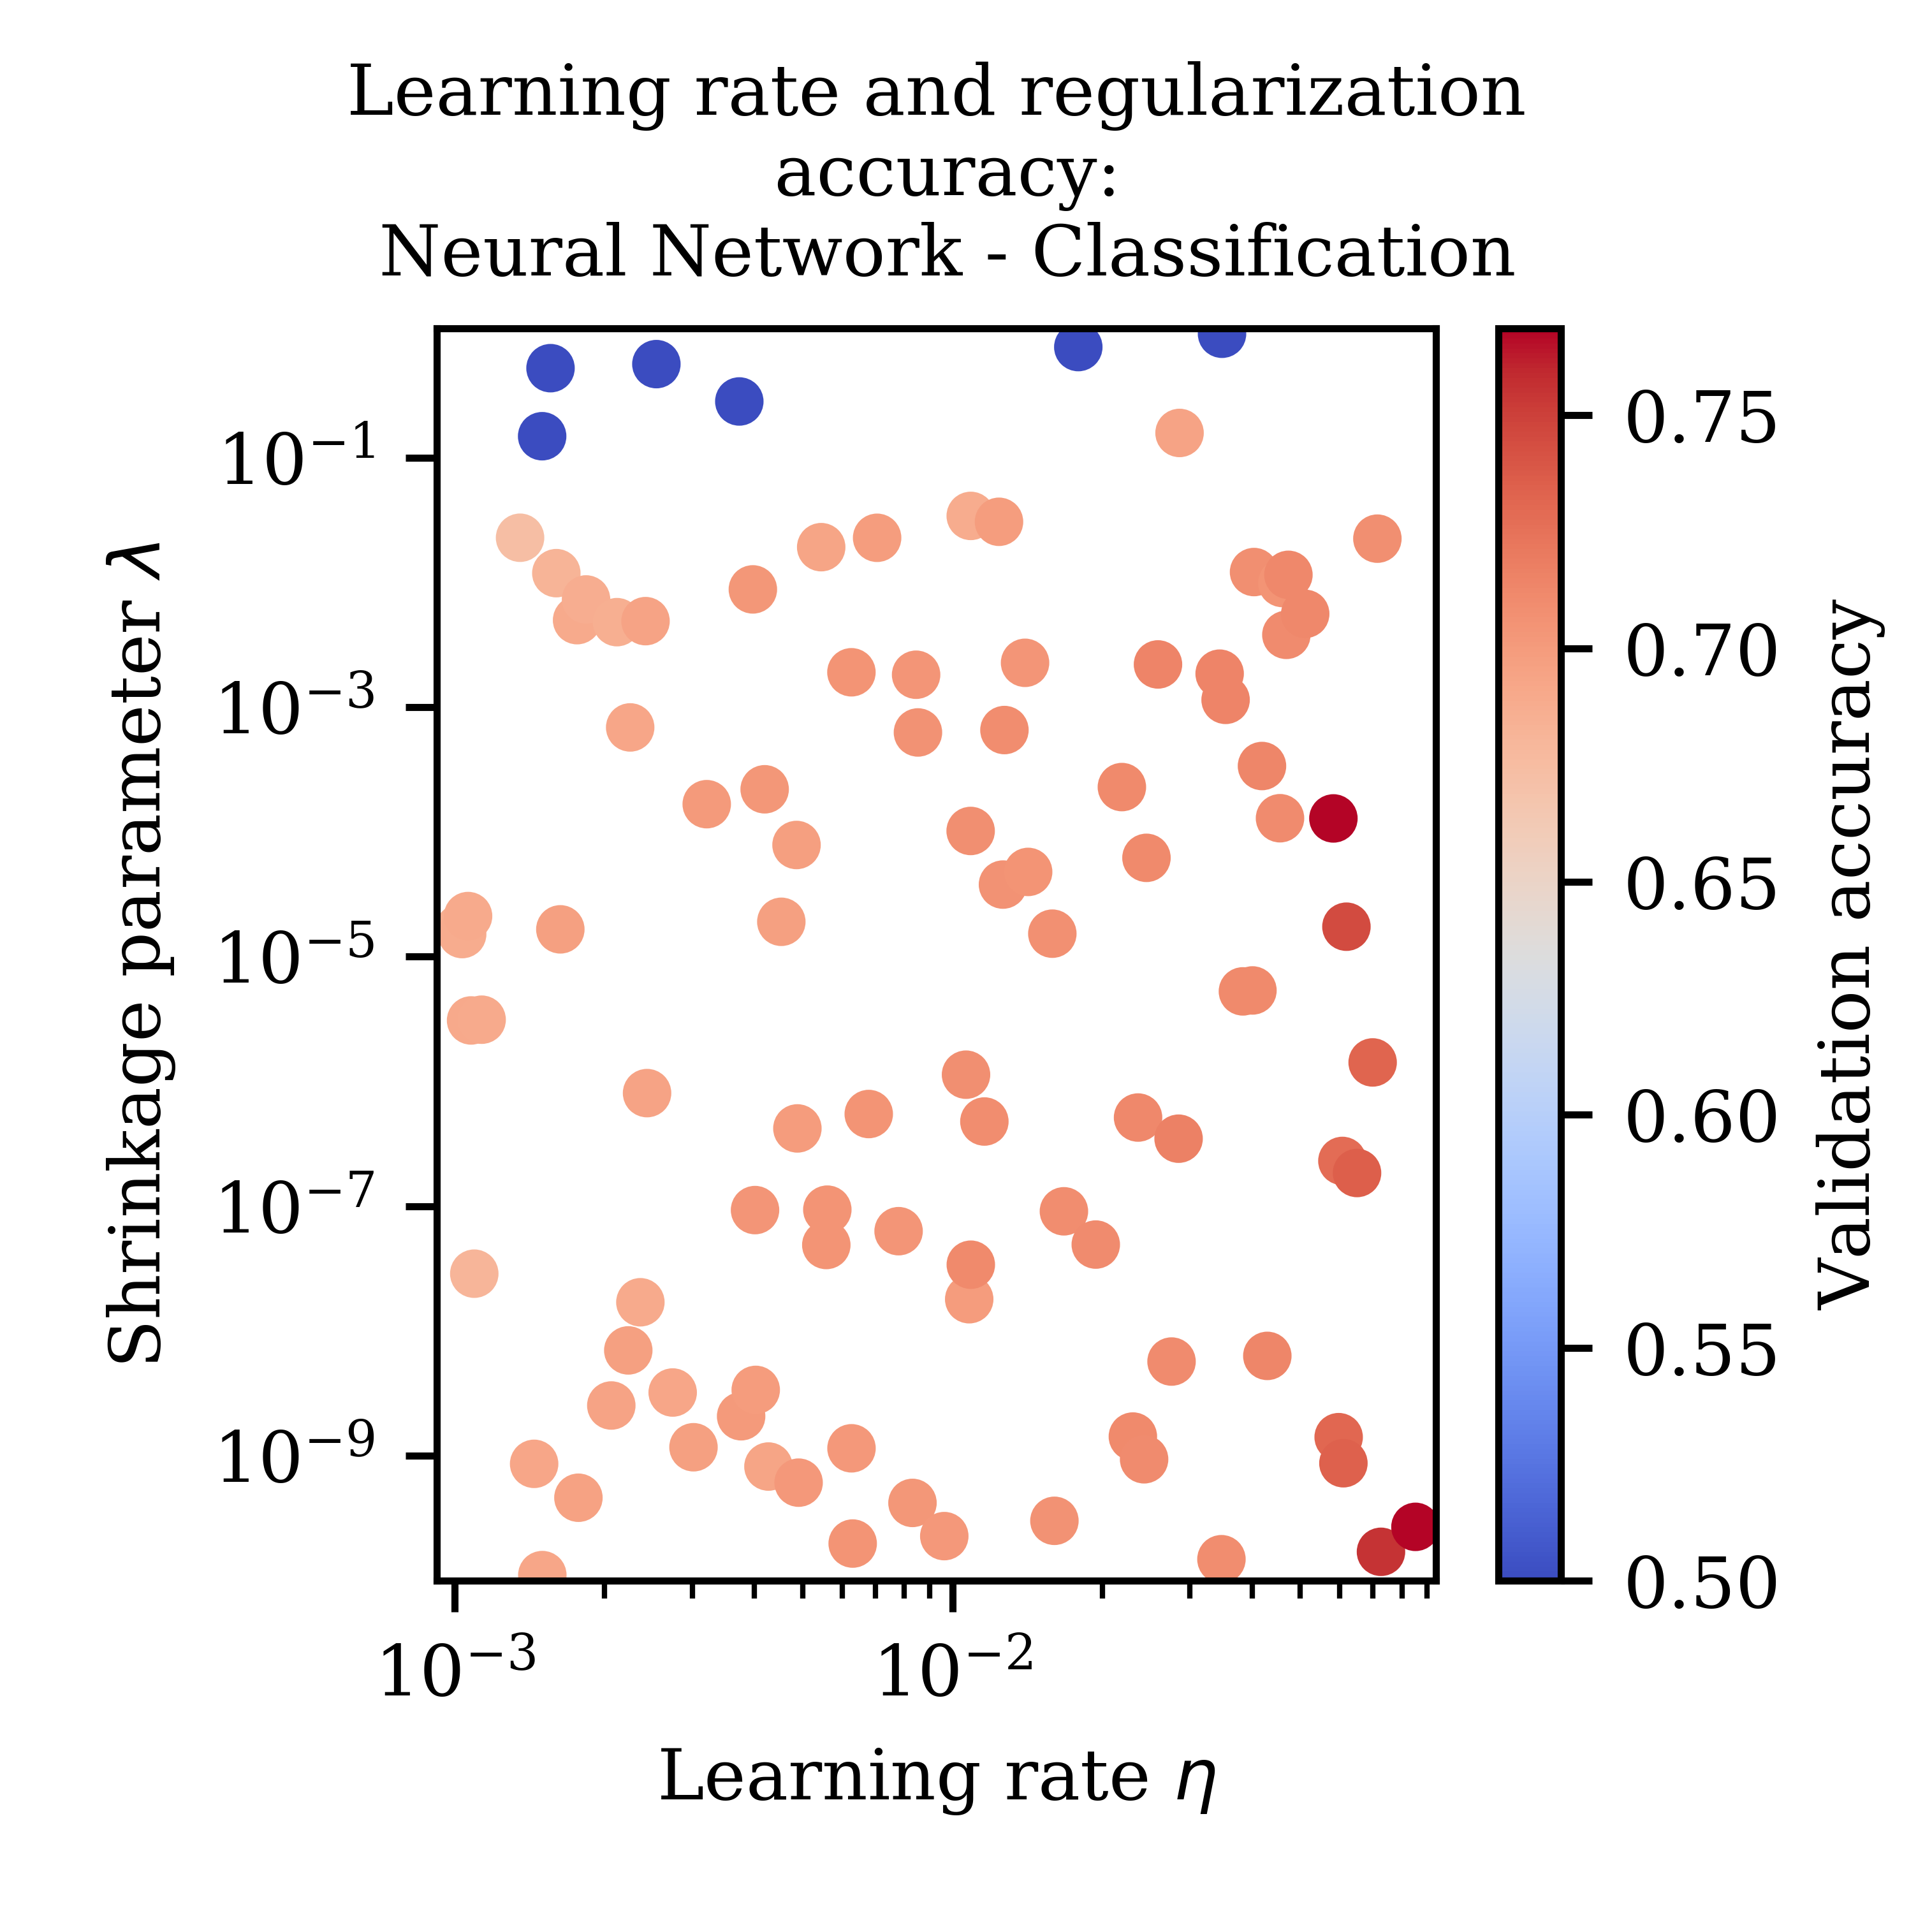
\includegraphics[width=0.5\linewidth]{nn_learning_rate_lambda_accuracy_credit.png}}
	\caption{This is visualizations of how the accuracy score changes with the learning rate and regularization parameter, to find the best values.\label{fig:class_best_params}}
\end{figure}
\begin{figure}[htbp]
	%\hspace*{-2.5cm}
	\subfloat[This is a plot of the cumulative gain for logistic regression fitting the credit card data as function of the number of samples.\label{subfig:LR_chart} ]{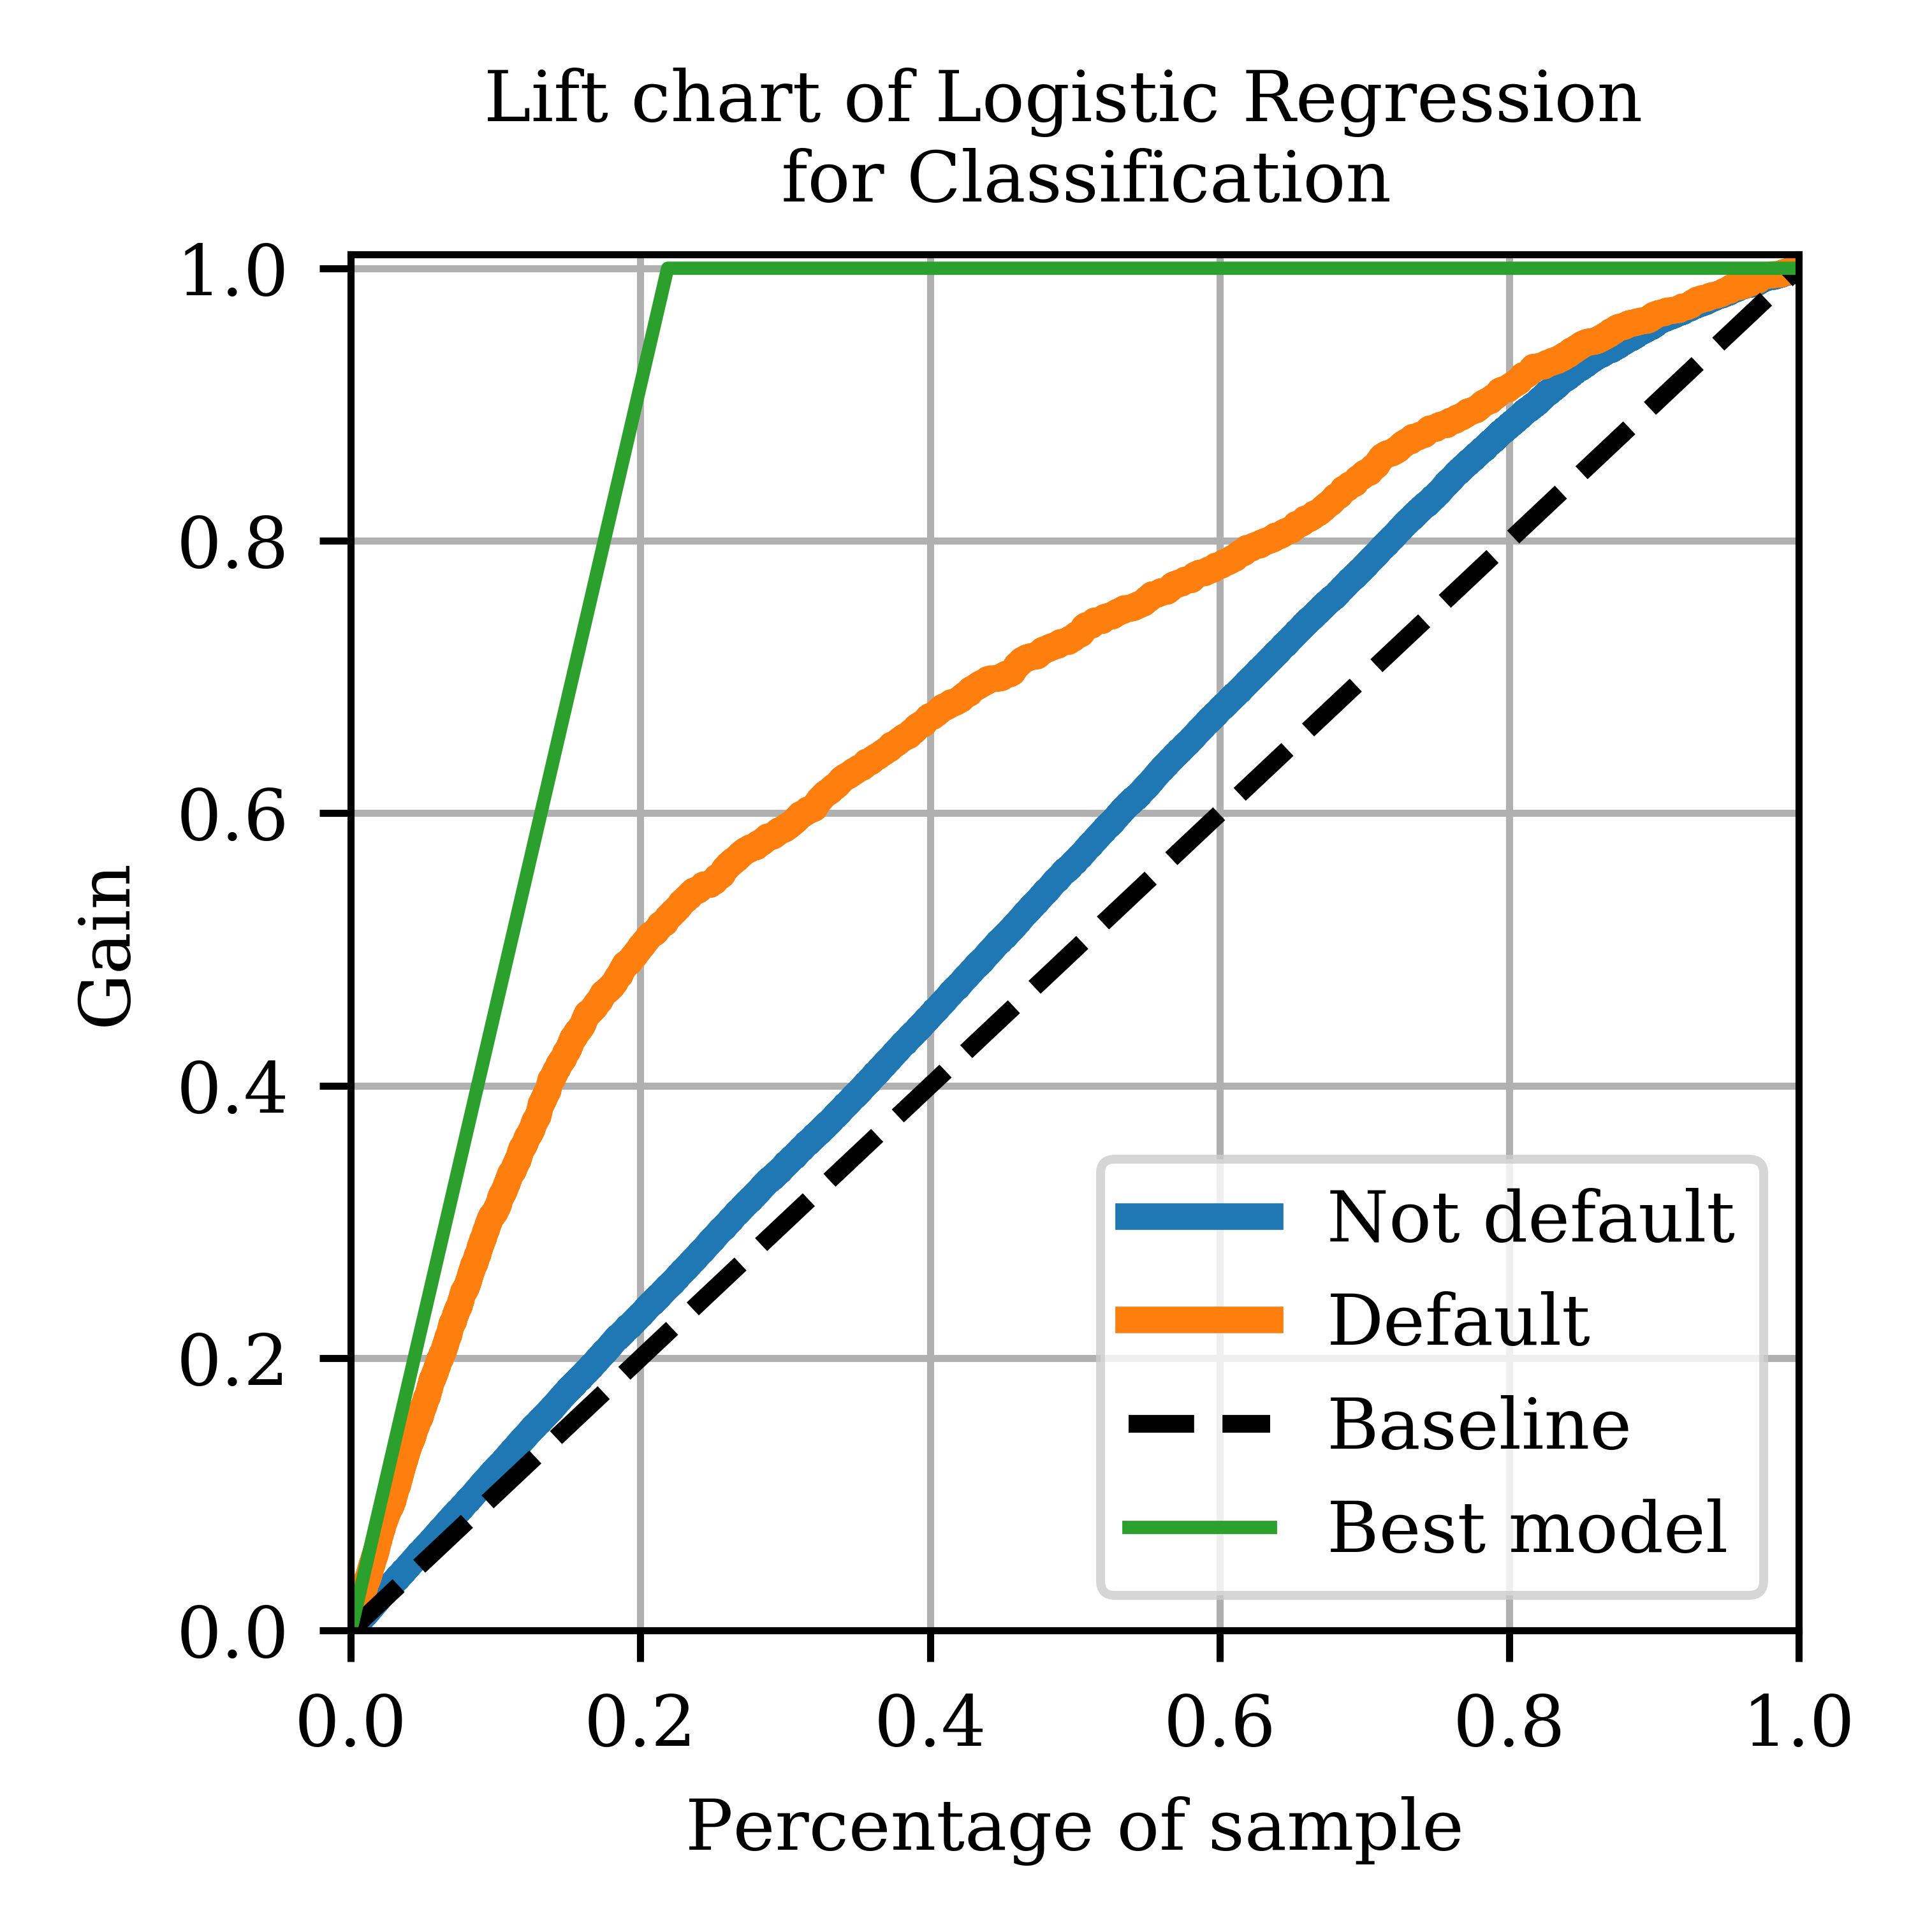
\includegraphics[width=0.5\linewidth]{cumulative_gain_logreg.png}}
	\hspace{0.5em}
	\subfloat[This is a plot of the cumulative gain for neural network fitting the credit card data as function of the number of samples.\label{subfig:NN_chart} ]{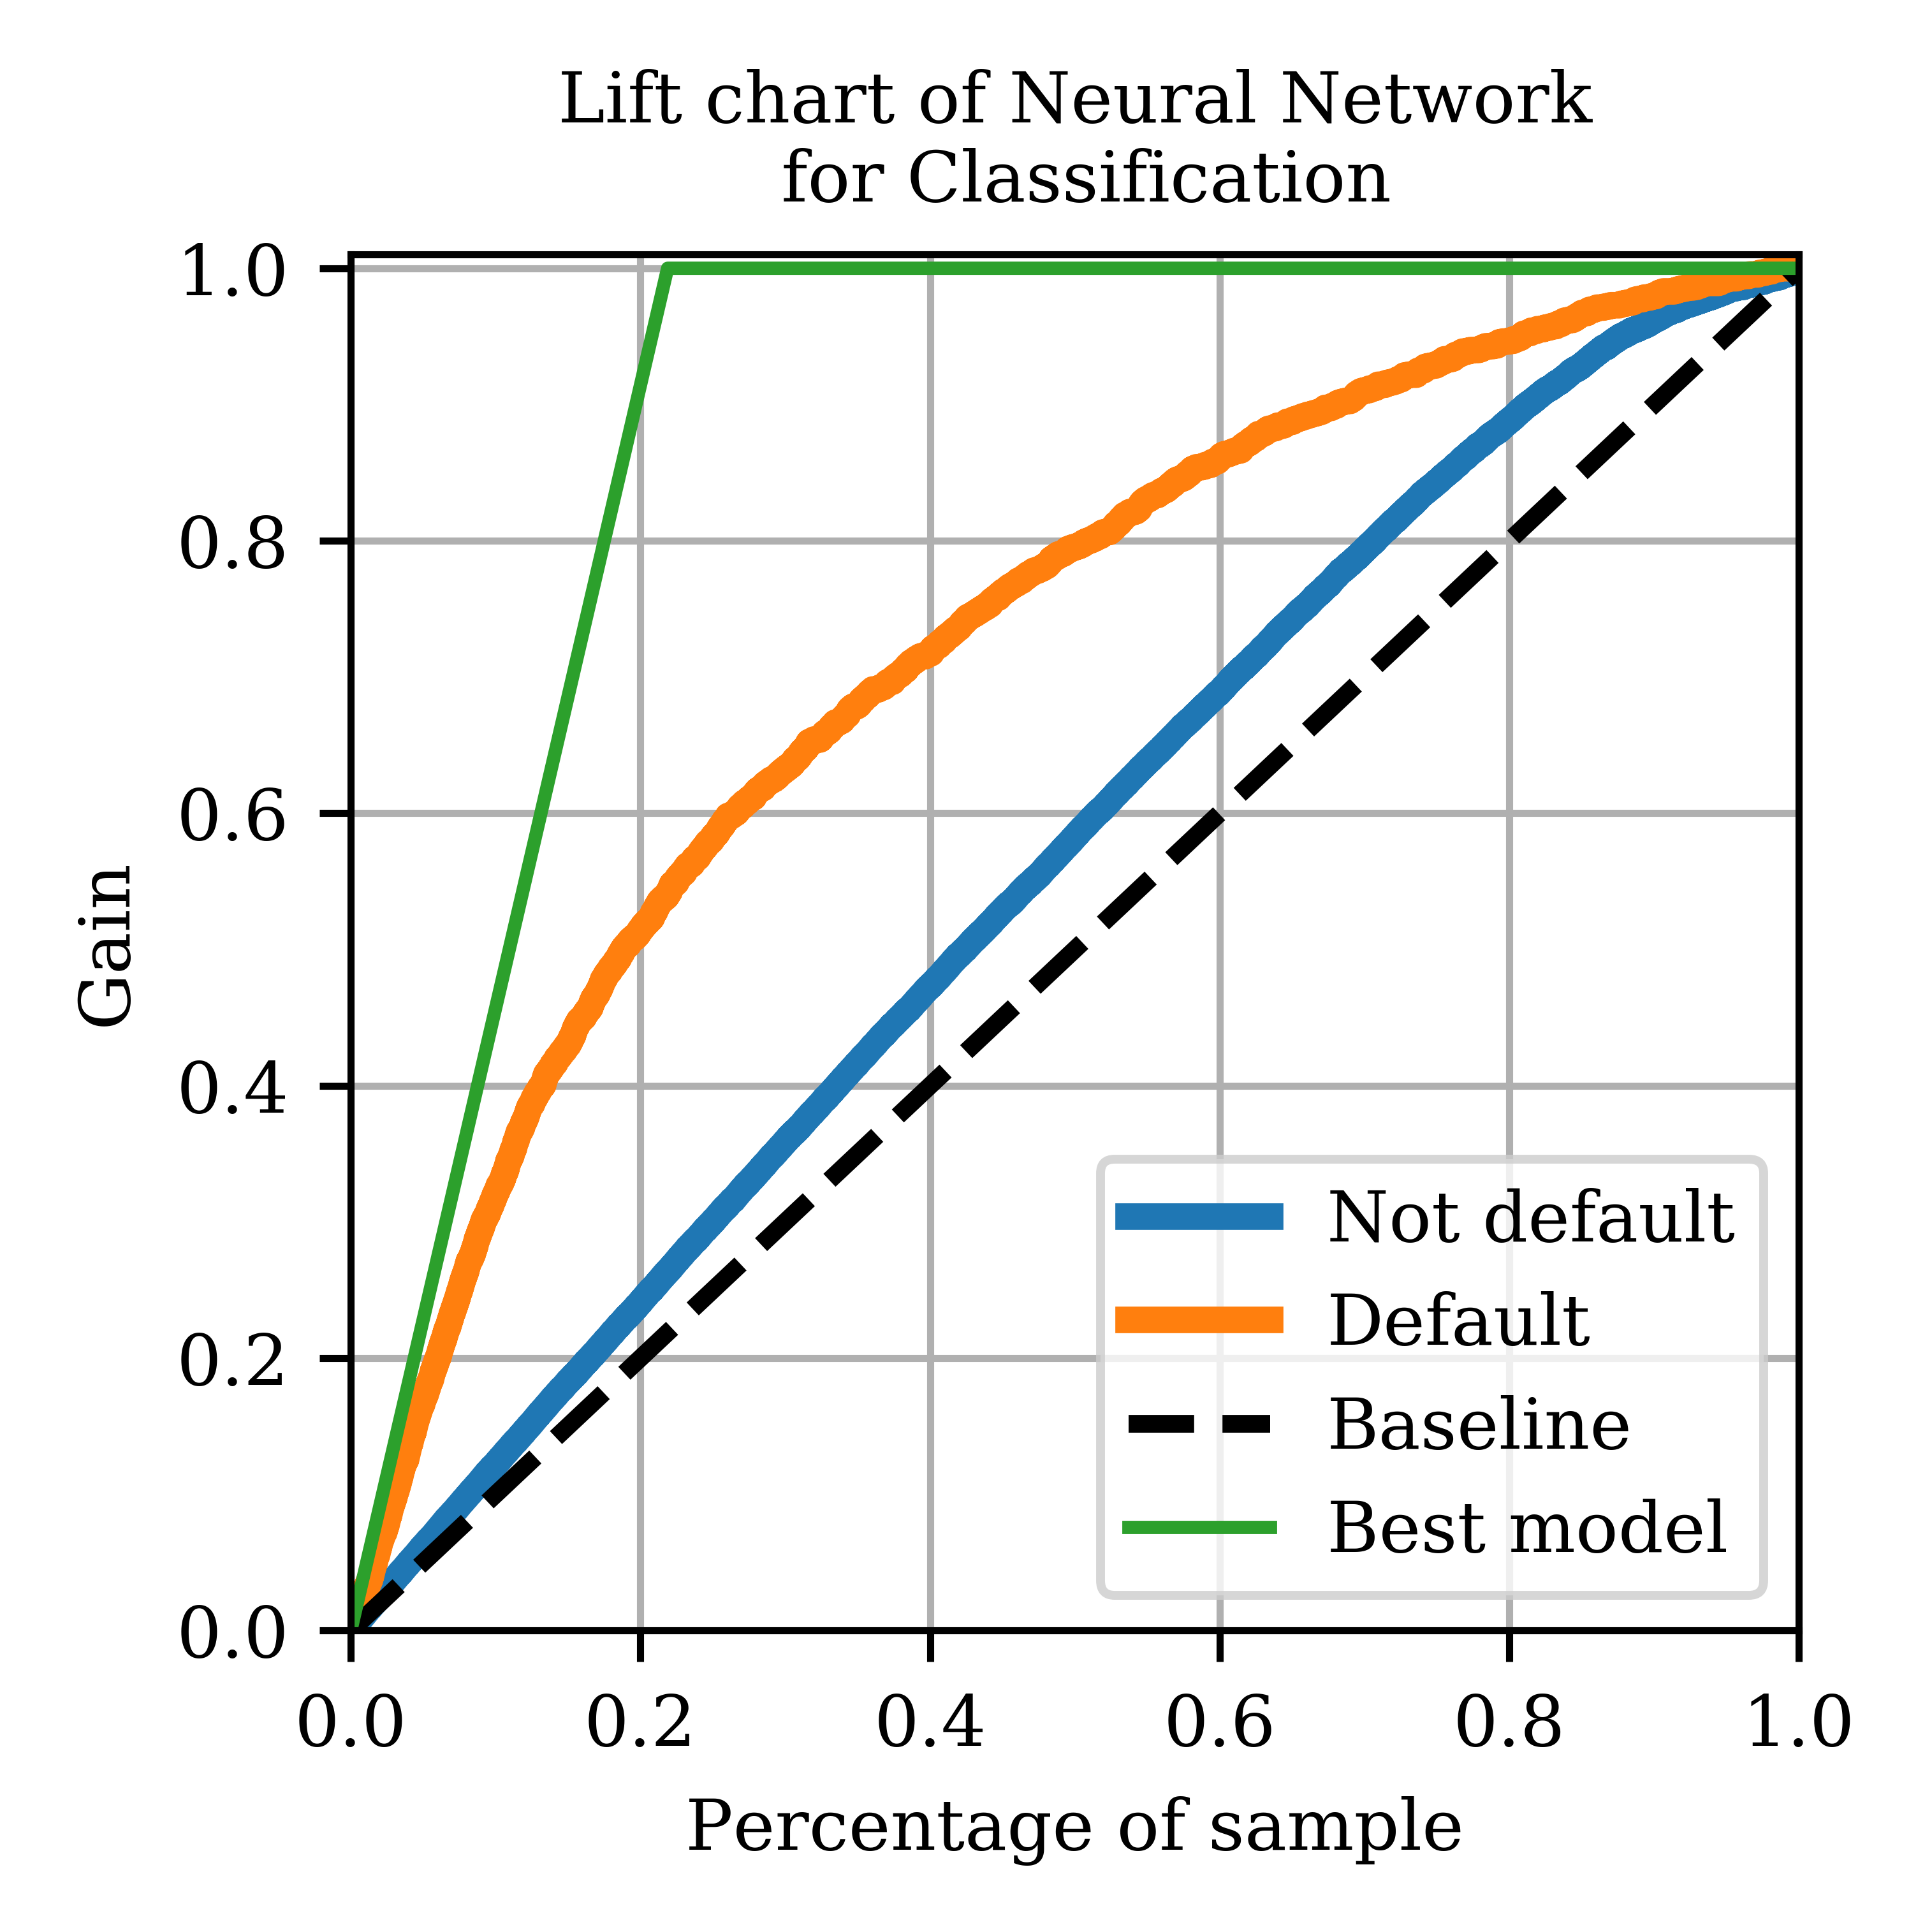
\includegraphics[width=0.5\linewidth]{cumulative_gain_NN.png}}
	\caption{Lift charts for logistic regression and neural network for classification. By comparing the two sub-figures, we can see that especially the default curve is closer to the best model for NN. This is the same as that the area ratio for the NN is higher than for LR. This can also be seen in Table \ref{tab:logreg}. So NN method looks like to be a better fit than the LR method for the credit card classification.\label{fig:class_lift_charts}}
\end{figure}

\subsection{Regression}
\label{subsect:result_reg}
In Table \ref{tab:reg} we see the $R^2$ scores for the training and test data, best learning rate and best regularization parameter for NN and OLS in the regression case for the given number of grid points $n_i$ and STD $\sigma$. In Figure \ref{fig:reg_best_params} we see the $R^2$ validation (test) scores for NN with $n_x=n_y=50, \sigma=0.2$ and $n_x=n_y=100,\sigma=0.1$. The best values for the hyperparameters are once again found numerically as in the classification case, and can be seen in Table \ref{tab:reg}. In Figure \ref{subfig:NN_low} we see that the $R^2$ score increases as the both the learning rate and regularization parameter decreases, but it starts to increase when the learning rate gets close to $10^{-5}$. So the $R^2$ score is also dependent on the learning rate, where the regularization parameter does not seem to affect the score as much in this case either. So to increase the fit we could most likely increase the model complexity, but this would increase the CPU time which already is quite high compared to the OLS.

In Figure \ref{fig:reg_fit} we see 3D plots of the Franke function fitted with NN for the two cases of parameters mentioned above with both the training and test data. The dots represents the regression model we get with the NN, while curves are the true Franke function data with added noise term $\mathcal{N}(0,\sigma^2)$. There it looks like Figures \ref{subfig:franke_100_train} and \ref{subfig:franke_100_test} give a better fit than the other case. This seems right since the total number of grid points is much higher here, so the fit has many more points to go after. We can also see this in Table \ref{tab:reg} by looking at the $R^2$ scores for the two cases.

For comparing the $R^2$ scores for the the first NN model and the OLS in Table \ref{tab:reg} (since they have the same input parameter values), we see that the OLS method is better than the NN. So the OLS in linear regression outperforms the NN regression in this case. If we increase the number of grid points and decrease the noise term, we see that the $R^2$ score increases a lot. So this gives a better fit for the Franke data when we increase the number of data points. This change give us a big increase in the CPU time as well. For the smaller number of grid points the CPU time was around 8 minutes, while for the bigger grid the time increased to around 40 minutes. One thing which is not tested is to run the OLS with the same parameters as the last NN with 10 000 grid points. This would most likely increase the $R^2$ score of the OLS. So the better method seems to be the OLS, which is a simple method that does not take nearly as long as the NN calculations.

\begin{table}[htbp!]
	\centering
	%\hspace{-1cm}
	\begin{tabular}{ |c|c|c|c| }
		\hline \rule{0pt}{13pt}
		& Neural Network  & Neural Network  & OLS  \\
		& $n_x=n_y=50$ & $n_x=n_y=100$ & $n_x=n_y=50$ \\
		& $\sigma=0.2$ & $\sigma=0.1$ & $\sigma=0.2$ \\
		\hline \rule{0pt}{13pt}
		$R^2$ score (test) & 0.551205 & 0.814861 & 0.680520 \\
		\hline \rule{0pt}{13pt}
		$R^2$ score (train) & 0.594956 & 0.820223 & - \\
		\hline \rule{0pt}{13pt}
		Best learning rate, $\gamma$ & 3.947107$\cdot10^{-4}$ & 5.8293$\cdot10^{-2}$ & - \\
		\hline \rule{0pt}{13pt}
		Best regularization parameter, $\lambda$ & 2.045894$\cdot10^{-7}$ & 1.285610$\cdot10^{-4}$ & - \\
		\hline
	\end{tabular}	
	\caption{Table for regression case for neural network and linear regression with ordinary least squares (OLS) on the Franke function data with the given parameters. $n_x$ and $n_y$ are the number of grid points in the x- and y-direction respectively, while $\sigma$ is the standard deviation (STD) in the added Gaussian noise term. Here we see that for the same parameters, the OLS is the better fit to the Franke data than the NN fro regression. By increasing the number of grid points from 2500 to 10 000 and decreasing the STD to 0.1, the $R^2$ score is increased by a lot. This also heavily increases the CPU time from around 8 minutes to around 40 minutes for running the randomized cross-validation search for the hyperparameters (sect. \ref{subsect:tuning}).}
	\label{tab:reg}
\end{table}
\begin{figure}[htbp]
	%\hspace*{-2.5cm}
	\subfloat[Here we see a heatmap of the $R^2$ score for the neural network regression case as function of the regularization parameter and learning rate with $n_x=n_y=50$ and $\sigma=0.2$. This is a visualization of how to find the best learning rate and best regularization parameter to be used in the neural network. Here we see that the best values are around $\lambda=10^{-10}-10^{-5}$ and $\gamma=10^{-5}-10^{-3}$.\label{subfig:NN_low} ]{\includegraphics[width=0.5\linewidth]{nn_learning_rate_lambda_r2_franke_50_50_0_2.png}}
	\hspace{0.5em}
	\subfloat[Here we see a heatmap of the $R^2$ score for the neural network regression case as function of the regularization parameter and learning rate with $n_x=n_y=100$ and $\sigma=0.1$. This is a visualization of how to find the best learning rate and best regularization parameter to be used in the neural network. Here we see that the best values are around $\lambda=10^{-9}-10^{-5}$ and $\gamma=10^{-5}-10^{-3}$. \label{subfig:NN_high} ]{\includegraphics[width=0.5\linewidth]{nn_learning_rate_lambda_r2_franke_100_100_0_1.png}}
	\caption{This is visualizations of how the accuracy score changes with the learning rate and regularization parameter, to find the best values.\label{fig:reg_best_params}}
\end{figure}
\begin{figure}[htbp]
	%\hspace*{-2.5cm}
	\subfloat[3D plot of the Franke function with STD $\sigma=0.2$ and total number of grid points 2 500 for the training data.\label{subfig:franke_50_train} ]{\includegraphics[width=0.5\linewidth]{3dplot_train_50_50_0_2.png}}
	\hspace{0.5em}
	\subfloat[3D plot of the Franke function with STD $\sigma=0.2$ and total number of grid points 2 500 for the test data. \label{subfig:franke_50_test} ]{\includegraphics[width=0.5\linewidth]{3dplot_test_50_50_0_2.png}}\\
	\subfloat[3D plot of the Franke function with STD $\sigma=0.1$ and total number of grid points 10 000 for the training data.\label{subfig:franke_100_train} ]{\includegraphics[width=0.5\linewidth]{3dplot_test_100_100_0_1.png}}
	\hspace{0.5em}
	\subfloat[3D plot of the Franke function with STD $\sigma=0.1$ and total number of grid points 10 000 for the test data. \label{subfig:franke_100_test} ]{\includegraphics[width=0.5\linewidth]{3dplot_test_100_100_0_1.png}}
	\caption{Here we see 3D plots of the Franke function data with added noise $\mathcal{N}(0,\sigma^2)$ fitted on the training and test sets. The dots represents the regression model we got from the neural network calculations. Here we see that is looks like the bottom two figures fits the data more. This is reasonable since they have a much higher $R^2$ score in Table \ref{tab:reg}.\label{fig:reg_fit}}
\end{figure}

\section{Conclusion}
In this project we have used logistic regression and neural network to analyze a binary classification case for credit card data, and to analyze a regression case for data sets produced by the Franke function (eq. \ref{eq:Franke_func}). For these data sets we have calculated how well the models fits to the data sets by the accuracy score (eq. \ref{eq:accuracy_score}) for classification and $R^2$ score (eq. \ref{eq:R2_score}) for regression. These results were then compared between the methods we have used, the results in a similar scientific paper \cite{origarticle} and the results in a previous project \cite{proj1} for linear regression on the Franke function. From all this calculations we can conclude that in this case the neural network (NN) works better for classification than logistic regression (LR). We got a higher accuracy score and area ratio for NN, around 0.795 and 0.566, than for LR, around 0.714 and 0.470. This corresponds quite well with the results in the scientific paper, which also concludes that neural network is better than logistic regression for classification. Even though the NN gives a better fit to the credit card data, it is a computer heavy model which also can be difficult to fully interpret. In the regression case, we found that linear regression with ordinary least squares (OLS) and $n_x=n_y=50, \sigma=0.2$ gives a better fit than the NN. The NN gave a $R^2=0.551$ while the the OLS gave $R^2=0.681$. Linear regression is also a much simpler model to both implement and to understand than neural network.

In the future we could try out other methods for classification like decision trees or gradient boosting. Especially gradient boosting is a hot topic in statistical physics today. They seem to be in the most cases very effective and maybe one of the best methods for classification cases today. Alternatively, we could try to improve our neural network code by changing different parameters like hidden layers, number of nodes etc. We could also try out different gradient solvers or activation functions to see how they affect the calculations.

\appendix
\section{Appendix}
\label{sect:Appendix}
Link to GitHub repository:\\
\url{https://github.com/krilangs/FYS-STK4155/tree/master/Project2}

\bibliographystyle{plainnat}
\bibliography{myrefs}
\end{document}